% Version 0.2
\documentclass[a4paper]{scrreprt}
 
\usepackage[german]{babel}
\usepackage[utf8]{inputenc}
\usepackage[T1]{fontenc}
\usepackage{ae}
\usepackage[bookmarks,bookmarksnumbered]{hyperref}
\usepackage{graphicx}
\usepackage{tabularx}
 
\begin{document}
 
\title{Visualisierung von \\ Whole Genome Alignments \\ mit der wgaPipeline}
\author{Sonja Hohlfeld}
\maketitle
 
\newpage 
% Platzierung des Inhaltsverzeichnisses
\tableofcontents
 
\chapter{Zielbestimmung}
\section{Musskriterien}
Die wgaPipeline soll eine Grafik erzeugen, die für die visuelle Darstellung eines Whole Genome Alignments (paarweise oder multiple) genutzt werden kann. Die Grafik soll folgende Eigenschaften des Alignments abbilden: 
\begin{itemize}
  \item Gene, die sich auf den Sequenzen befinden, sollen farblich auf dem entsprechenden DNA-Strang hervorgehoben werden.
  \item Das Verwandschaftsverhältnis der zu untersuchenden Sequenzen soll mit einem Stammbaum visualisiert werden.
  \item Eine angemessene Beschriftung, der Sequenzen und der Gene.
  \item Übereinstimmende Motive zwischen den Sequenzen sollen mit einem Farbcode für die entsprechenden Identitäten dargestellt werden.
\end{itemize}
Darüber hinaus soll die Sofware mit folgenden interaktiven Features ausgestattet werden:
\begin{itemize}
  \item Ein beliebiger Wechsel zwischen linearem und zirkulärem Layout. 
  \item Der Benutzer besitzt die Möglichkeit, die Grafik zu konfigurieren. 
  \item Mit einem Slider kann die Mindestlänge oder -identität der übereinstimmenden Sequenzmotive gefiltert werden. Dabei sollte sich das Maximum des Längensliders flexibel an die maximale Länge der Sequenzmotive anpassen.
\end{itemize}

\section{Kannkriterien}
Damit der Benutzer noch besser mit der wgaPipeline interagieren kann, wären weitere dynamische Möglichkeiten der Software wünschenswert z.B.:
\begin{itemize}
  \item Der Benutzer kann alle Sequenzen des Alignments flexibel in der Grafik verschieben und neu sortieren.
  \item Zoom feature: kleine Regionen einer langen Sequenz können markiert und dann detailliert abgebildet werden.
  \item Diagramm, dass den GC-Gehalt und die read-Coverage darstellt
\end{itemize}
Zudem wäre es sinnvoll noch mehr biologische Merkmale der Gene und der Sequenzen abzubilden z.B:
\begin{itemize}
  \item Repeats, inverted repeats 
  \item tRNAs, coding sequences, introns
  \item Merkmale, die durch den Benutzer definiert werden können
\end{itemize}

\newpage
\section{Abgrenzungskriterien}
Die wgaPipeline ist keine Software für die Berechnung von Stammbäumen. Das heißt es gibt keine Möglichkeit einen Stammbaum auf Basis des Alignments berechnen zu lassen. Der Stammbaum wird nur gezeichnet, wenn der Benutzer die dafür notwendigen Daten vor Erstellung der Grafik dem Programm übergibt.

Darüber hinaus liegt es nicht in meinem Aufgabenbereich, die Berechnung des Aligments durchzuführen und daraus die Daten zu generieren. Für die Visualisierung des Alignments bekomme ich lediglich den fertigen Datensatz in Form eines JSON-Files, das alle notwendige Informationen über Features, Links und Karyo enthält.

\chapter{Einsatz} 
\section{Anwendungsbereiche}
Die wgaPipeline wird für biologische Sequenzanalysen genutzt. Dabei werden die Ergebnisse eines Alignments klar und übersichtlich in einer Abbildung visualisiert. Auf Basis dieser Grafik sind beispielsweise Aussagen über evolutive Vorgänge auf molekularer Ebene, RNA-Faltungsprozesse oder die Vorhersage räumlicher Proteinstrukturen anhand bereits bekannter Proteine mit ähnlichen Sequenzen möglich. 

\section{Zielgruppen}
Die Zielgruppe besteht aus Biologen, die sich im Rahmen einer Sequenzanalyse mit einer biologischen Fragestellung beschäftigen und ihre Ergebnisse in einer übersichtlichen Abbildung darstellen möchte. Die Abbildung kann für Protokolle, wissenschaftlische Arbeiten, Publikationen, etc. genutzt werden.

\section{Betriebsbedingungen}
Für die Visualisierung des Alignments wird ein Browser benötigt.

\chapter{Umgebung} 
\section{Software}
Für die Darstellung der Abbildung wird ein Browser benötigt, der JavaScript zulässt.
\section{Hardware}
s. Software
\section{Orgware}
Zunächst muss der bereits exisitierende Code in Bezug auf Objekt-Orientierung umstrukuriert werden und alle bereits geschriebenen Funktionen müssen wieder funktionieren, sodass die Grafik vollständig wieder hergestellt ist.

Parallel dazu, müssen die Tests erweitert und den neuen Funktionen angepasst werden. Dabei soll die angestrebte Coverage mindestens 75\% betragen. 

Zuletzt wird ein entsprechender Testdatensatz benötigt, der einerseits mehrere Sequenzen einer genomeID, andererseits auch mehrer genomeIDs enthält, damit auch die Darstellung eines multiplen Alignments möglich ist. Darüber hinaus müssen die Daten Stammbauminformationen sowie Informationen über auf den Sequenzen liegende Gene enthalten. 
\chapter{Funktionalität}
\section{Alignmentvisualisierung im linearen und zirkulären Layout}
Die Visualisierung des Alignments erfolgt in einem zirkulären oder einem linearen Layout. Der Benutzer soll in der Lage sein, per Button die Darstellungsform zu wechseln.
\section{Darstellung von Genen}
Für erweiterte Analyseoptionen sollen alle Gene, die sich auf den Sequenzen befinden, strangspezifisch dargestellt werden. 
\section{Beschriftung von Sequenzen und Genen mit Legende}
Alle Sequenzen und Gene sollen beschriftet werden. Im Moment ist noch nicht klar, ob die Beschriftung der Sequenzen mit einem Tooltip erfolgt oder fest gesetzt wird. Eventuell werden auch beide Optionen in der Grafik angeboten.

Zudem sollen für eine verbesserte Übersichtlichkeit alle Gene nur mit Hilfe einer Legende beschriftet werden.

\section{Visualisierung des Verwandschaftsverhältnisse mit einem Stammbaum}
Ein Stammbaum soll das Verwandschaftsverhältnis der zu untersuchenden Sequenzen darstellen. Die dafür benötigten Daten werden vom Benutzer mitgegeben und eine entsprechende Funktion zeichnet den Stammbaum. 

Der Benutzer soll die Möglichkeit haben, die Reihenfolge der Sequenzen im Stammbaum durch Mouseclick auf die Knotenpunkte individuell zu verändern.

\section{Konfigurationsmöglichkeiten für den Benutzer durch Interaktivität der Grafik}
Damit der Benutzer die Möglichkeit besitzt, die Grafik seinen individuellen Wünschen anzupassen, sollen verschiedene Funktionen die Grafik konfigurierbar machen.

Zunächst soll die Beschriftung flexibel sein. Das heiß, der Benutzer kann entscheiden, ob er die fest gesetzten Beschriftungen der Sequenzen sowie die Legenden angezeigt haben möchte.

Es soll die Möglichkeit bestehen, die Farben der gezeichneten Sequenzen und der Gene zu verändern.

Außerdem kann der Farbcode für die übereinstimmenden Sequenzmotive individuellen Wünschen angepasst werden. So soll eine beliebig definierte Abstufung des Farbcodes möglich sein .

Mit Hilfe von Slidern soll der Benutzer in der Lage sein, die Sequenzmotive hinsichtlich Mindestlänge und -identität zu filtern. Für eine verbesserte Flexibilität soll das Maximum des Längefilters an das längste übereinstimmende Sequenzmotiv angepasst werden.

\chapter{Daten}
Format und Inhalt der Daten, die der Benutzer benötigt um ein Alignment visualisieren zu können.
\section{karyo.tsv}
\begin{tabular}{|c|c|c|}\hline
   chr & genomeID & length \\ \hline
   chr1 & 0 & 10000 \\ \hline
   chr2 & 1 & 6000 \\ \hline
   chr3 & 1 & 9000 \\ \hline
   chr4 & 2 & 9000 \\ \hline
\end{tabular}
\section{features.bed}
\begin{tabular}{|c|c|c|c|}\hline
   chr & start & end & featureID \\ \hline
   chr1 & 1000 & 6000 & L1a \\ \hline
   chr2 & 1000 & 5000 & L1b \\ \hline
   chr3 & 7000 & 9000 & L2a \\ \hline
   chr4 & 5500 & 7000 & L2b \\ \hline
\end{tabular}
\section{links.tsv}
\begin{tabular}{|c|c|c|}\hline
   fida & fidb & identity \\ \hline
   L1a & L1b & 94 \\ \hline
   L2a & L2b & 75 \\ \hline
   L2b & L1a & 80 \\ \hline
\end{tabular}


\chapter{Benutzungsoberfläche}
Die Grafik wird in einem Browserfenster präsentiert. Der aktuelle Stand ist in der folgenden Abbildung dargestellt.
\begin{figure}[h]
  \centering
  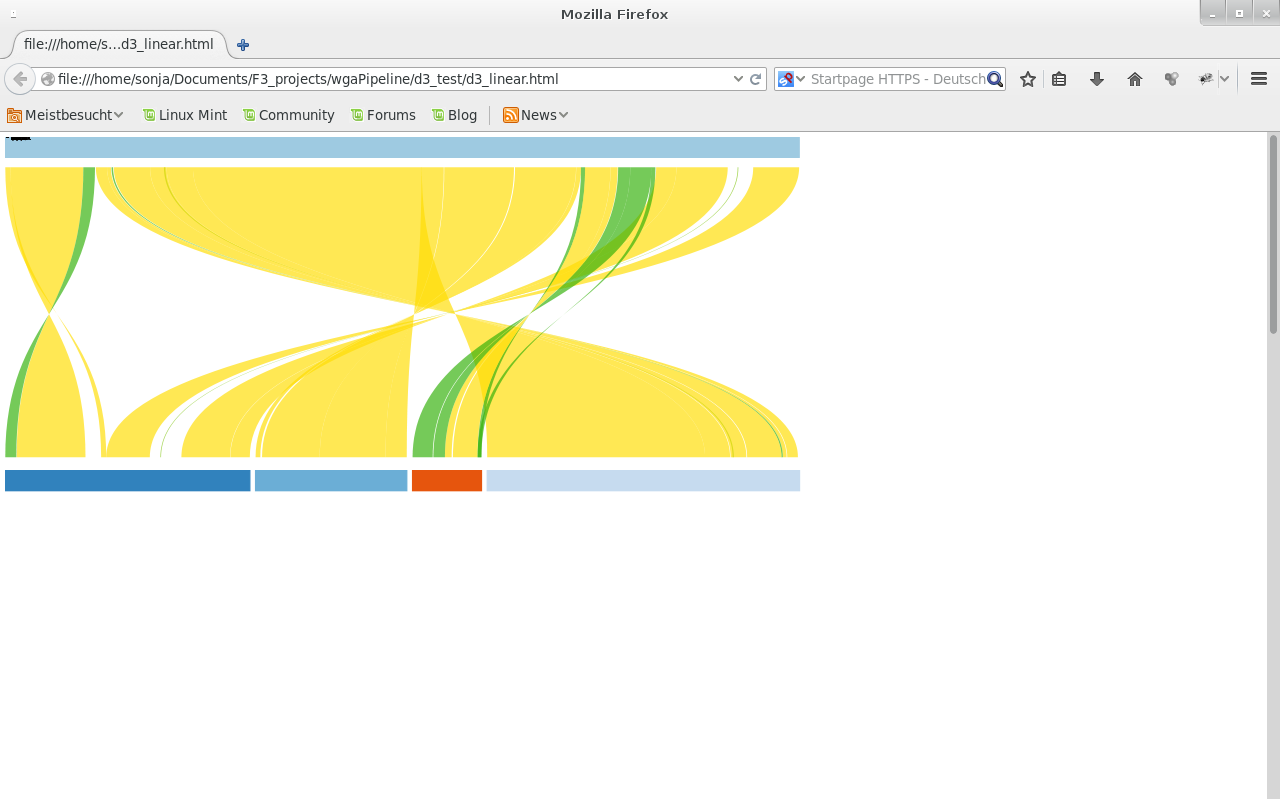
\includegraphics[width=11.5cm]{figures/linear.png}
  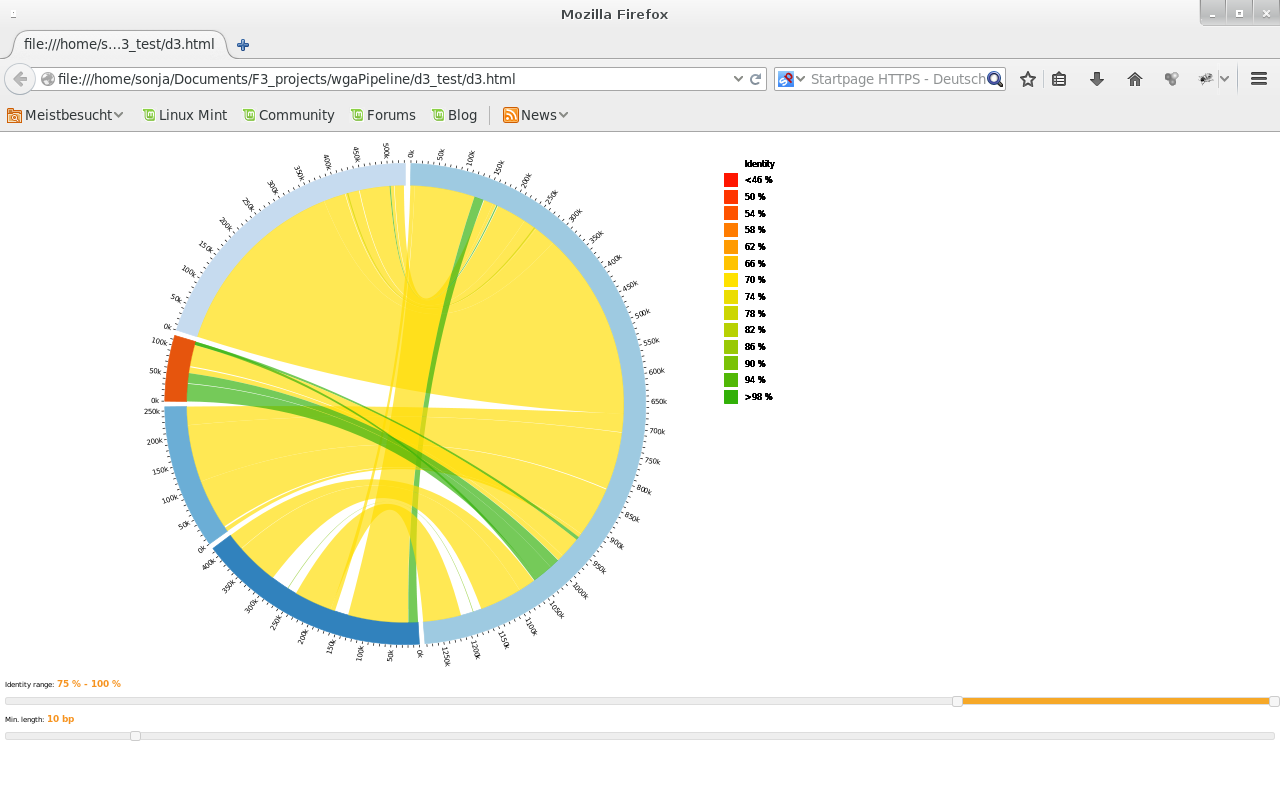
\includegraphics[width=11.5cm]{figures/circular.png}
  \caption{Lineare und zirkuläre Version der wgaPipeline im Browserfenster. Alle interaktiven Features sollen hier für den Benutzer aufrufbar sein.}
\end{figure}

Alle interaktiven Features sollen über diese Abbildung ausführbar sein.\\
Über den Slider kann der Benutzer die Mindestlänge und -identität der dargestellten Sequenzmotive regulieren.\\
Die flexible Erscheinung von Beschriftung und Legende soll durch Mouseclick auf Beschriftung und Legende möglich sein.\\
Auch die flexible Reihenfolge der Sequenzen in dem Stammbaum soll durch Mouseclicks auf die entsprechende Zeichnung interaktiv werden.




\chapter{Qualitätsziele}
Der Code für die Visualisierung des Alignments soll durch eine umfassende Testumgebung mit Jasmine, grunt und Travis CI auf seine korrekte Funktionsweise, einheitliche Syntax und sinnvolle Struktur geprüft werden. Die Coverage sollte dabei mindestens 75\% betragen.
 
% Abbildungsverzeichnis
\listoffigures
 
\end{document}
